\documentclass{standalone}

\usepackage{pgfmath}
\usepackage{pgf}
\usepackage{tikz}
% \usepackage{pgfplots}
% 	\usepgfplotslibrary{groupplots}
    \usetikzlibrary{calc}
    \usetikzlibrary{positioning}
    \usetikzlibrary{angles,quotes}
    \usetikzlibrary{backgrounds}
    \usetikzlibrary{external}
    \usetikzlibrary{fit}
    \usetikzlibrary{bayesnet}
    \usetikzlibrary{calc}
    \usetikzlibrary{fit}
    \usetikzlibrary{spy, shadows}
    \usetikzlibrary{arrows.meta}
    \usetikzlibrary{shadings}
    \usetikzlibrary{fadings}
    %\usetikzlibrary{tikzmark}
    \usetikzlibrary{matrix}
% all other packages and stuff you need for the picture
%
\newcommand*\circled[2]{\tikz[baseline=(char.base)]{
            \node[shape=circle,draw, #1] (char) {#2};}}

\begin{document}
\begin{tikzpicture}
\node(d0) {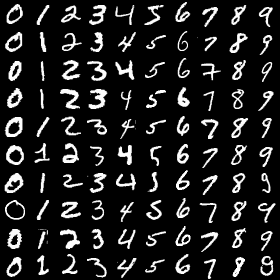
\includegraphics[scale=0.4, trim=0 101 0 0, clip, trim=0 101 0 0, clip]{figs/gen_samples/data_digit_plot.png}};
\node[below=-0.1 of d0] (f0){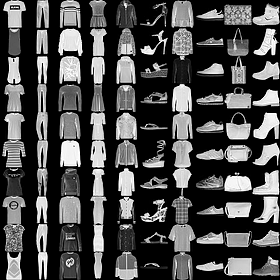
\includegraphics[scale=0.4, trim=0 101 0 0, clip]{figs/gen_samples/data_fashion_plot.png}};
\node[right=-0.1 of d0] (d1) {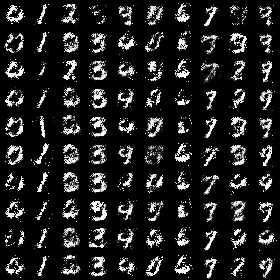
\includegraphics[scale=0.4, trim=0 101 0 0, clip]{figs/gen_samples/dp_cgan_digit_plot.png}};
\node[right=-0.1 of f0] (f1){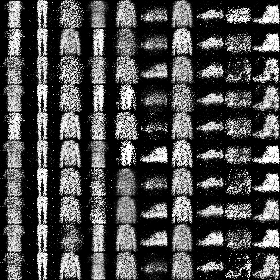
\includegraphics[scale=0.4, trim=0 101 0 0, clip]{figs/gen_samples/dp_cgan_fashion_plot.png}};
\node[right=-0.1 of d1] (d2) {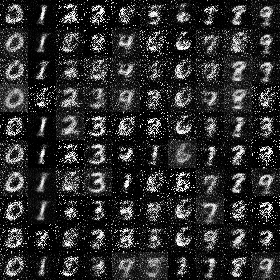
\includegraphics[scale=0.4, trim=0 101 0 0, clip]{figs/gen_samples/dmnist_direct_plot.png}};
\node[right=-0.1 of f1] (f2)  {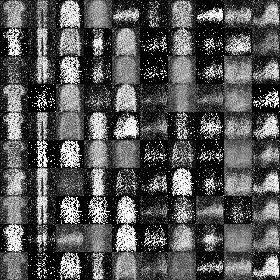
\includegraphics[scale=0.4, trim=0 101 0 0, clip]{figs/gen_samples/fmnist_direct_plot.png}};
\node[right=-0.1 of d2] (d3) {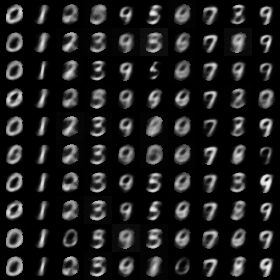
\includegraphics[scale=0.4, trim=0 101 0 0, clip]{figs/gen_samples/dp_ae_gmmn_digit_plot.png}};
\node[right=-0.1 of f2] (f3)  {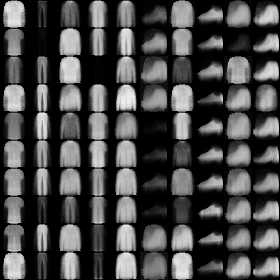
\includegraphics[scale=0.4, trim=0 101 0 0, clip]{figs/gen_samples/dp_ae_gmmn_fashion_plot.png}};
\node[anchor=center] at ($(f0.south)-(0.0,0.2)$) {Data Samples};
\node[anchor=center] at ($(f1.south)-(0.0,0.2)$) {DP-CGAN};
\node[anchor=center] at ($(f2.south)-(0.0,0.2)$) {DP-MERF};
\node[anchor=center] at ($(f3.south)-(0.0,0.2)$) {DP-MERF+AE};
\end{tikzpicture}
\end{document}
